\titlespacing*{\section}
{0pt}{1ex plus 1ex minus .2ex}{-2.3ex plus .2ex}
\newcommand{\skipper}{\medskip\hrulefill\section{}}

  
        \centering
        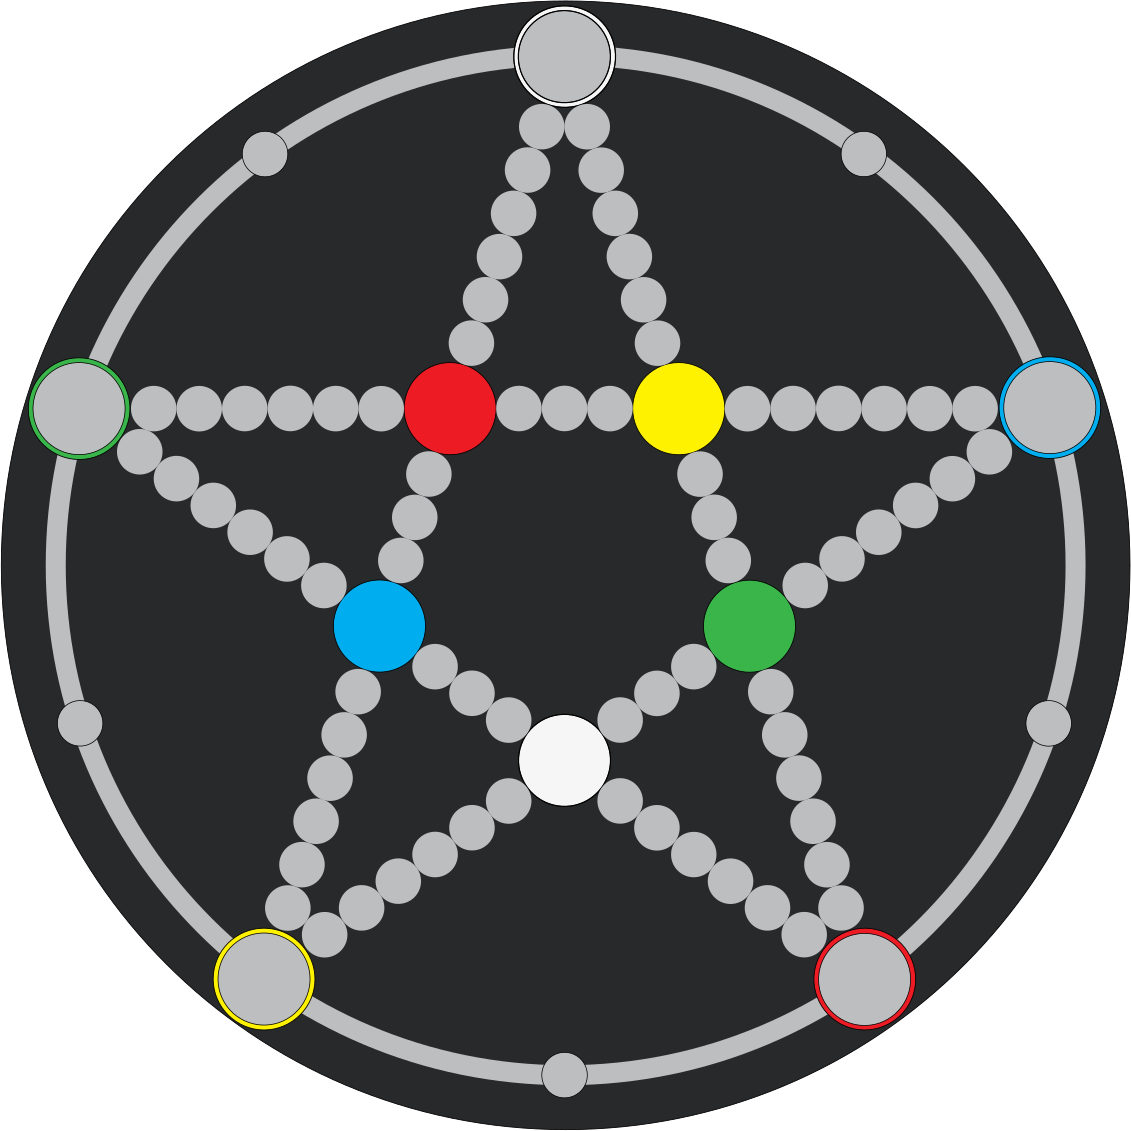
\includegraphics[width=0.5\textwidth]{Pentagame_board_2018.png}
        
        \vspace{6ex}
        
        {\sffamily\Large\textbf{PENTA$\cdot$GAME}}
        
        \bigskip

    \begin{enumerate}
    \centering
        \item Every player has one piece on each corner
        \item Black blocks sit on central nodes
        \item Goal: Reach the coloured nodes opposite
        \item Everything goes, but no jumping allowed
        \item Replace blocks, swap with pieces
        \item Upon moving out place a grey block
        \item Three pieces out wins
        \item Grey blocks are one time blocks
        \item No repetition (Ko)
    \end{enumerate}
    
\newpage



    \centering
    
    \skipper
    
    \begin{tikzpicture}[scale=0.65,state/.style={circle, draw, inner sep=2pt, opacity=1, fill=black, minimum size=0.2pt}]
    \tikzset{empty/.style={circle, draw, inner sep=2pt, opacity=0, fill=white, minimum size=0.2pt}}
    \tikzset{cross/.style={cross out, draw=black, minimum size=2*(#1-\pgflinewidth), inner sep=2pt, outer sep=2pt},
    %default radius will be 1pt. 
    cross/.default={1pt}}
    \scriptsize
    \begin{scope}[xscale=-1]
    \def \n {5} \def \radius {3cm} \def \raz {1.4cm}
    \foreach \s in {1,...,\n} { 
    \draw[dashed, >=latex] ({360/\n * (\s - 1)}:\radius)      arc ({360/\n * (\s - 1)}:{360/\n * (\s)}:\radius);   
    \draw[dotted, >=latex] ({360/\n * (\s - 2)+90}:\radius)      -- ({360/\n * (\s)+90}:\radius); 
    } 
    
    \node[state, fill=white] (1) at ({360/\n * (1 - 1)+90}:\radius) {};  
    \node[state, fill=white] (1a) at ({360/\n * (1 - 1)+90}:-\radius/2.618) {}; 
    
    \node[state, fill=blue] (2) at ({360/\n * (2 - 1)+90}:\radius){};   
    \node[state, fill=blue] (2a) at ({360/\n * (2 - 1)+90}:-\radius/2.618) {}; 
    
    \node[state, fill=red] (3) at ({360/\n * (3 - 1)+90}:\radius) {};  
    \node[state, fill=red] (3a) at ({360/\n * (3 - 1)+90}:-\radius/2.618) {}; 
    
    \node[state, fill=yellow] (4) at ({360/\n * (4 - 1)+90}:\radius) {}; 
    \node[state, fill=yellow] (4a) at ({360/\n * (4 - 1)+90}:-\radius/2.618) {}; 
    
    \node[state, fill=green] (5) at ({360/\n * (5 - 1)+90}:\radius) {};   
    \node[state, fill=green] (5a) at ({360/\n * (5 - 1)+90}:-\radius/2.618) {}; 
    
    
    \draw[>=triangle 45, line width=1.5pt, ->] (1) -- (1a) ;
    \end{scope}
    \end{tikzpicture}
    %\caption{Objective}
    
    You have five pieces.
    
    Bring them to the their \textbf{goals opposite their origins:}
    
    White to white, blue to blue etc.
    
    \textbf{Three out wins.}

% \begin{multicols}{2}
% \raggedcolumns



 
  
\skipper 

    \begin{tikzpicture}[scale=0.65,state/.style={circle, draw, inner sep=2pt, opacity=1, fill=black, minimum size=0.2pt}]
    \tikzset{empty/.style={circle, draw, inner sep=2pt, opacity=1, fill=white, minimum size=0.2pt}}
    \tikzset{cross/.style={cross out, draw=black, minimum size=2*(#1-\pgflinewidth), inner sep=2pt, outer sep=2pt},
    %default radius will be 1pt. 
    cross/.default={1pt}}
    \scriptsize
    \begin{scope}[xscale=-1]
    \def \n {5} \def \radius {3cm} \def \raz {1.4cm}
    \foreach \s in {1,...,\n} { 
    \draw[dashed, >=latex] ({360/\n * (\s - 1)}:\radius)      arc ({360/\n * (\s - 1)}:{360/\n * (\s)}:\radius);   
    \draw[dotted, >=latex] ({360/\n * (\s - 2)+90}:\radius)      -- ({360/\n * (\s)+90}:\radius); 
    } 
    %\draw[dashed] ({360/\n * (1 - 1)+95}:\radius)      arc ({360/\n * (1 - 1)+95}:{360/\n * (1)+85}:\radius)  node[midway, rotate=-18] {$\times$};
    \draw[>=triangle 45, line width=1.5pt, ->] ({360/\n * (1-1)+95}:\radius)  arc ({360/\n * (1-1)+95}:{360/\n * (2-1)+80}:\radius) node[midway,left]{};
    
    \draw[>=triangle 45, line width=1.5pt, ->] ({360/\n * (1-1)+95}:\radius)  arc ({360/\n * (1-1)+95}:{360/\n * (-1)+100}:\radius) node[midway,left]{};
    
    \draw[>=triangle 45, line width=1.5pt, shorten >=1.5ex, ->] (1) -- (4a);
    
    \draw[>=triangle 45, line width=1.5pt, shorten >=1.5ex, ->] (1) -- (3a);
    
    
    \node[state, fill=white] (1) at ({360/\n * (1 - 1)+90}:\radius) {};  
    \node[state, fill=white] (1a) at ({360/\n * (1 - 1)+90}:-\radius/2.618) {}; 
    
    \node[state, fill=blue] (2) at ({360/\n * (2 - 1)+90}:\radius){};   
    \node[state, fill=blue] (2a) at ({360/\n * (2 - 1)+90}:-\radius/2.618) {}; 
    
    \node[state, fill=red] (3) at ({360/\n * (3 - 1)+90}:\radius) {};  
    \node[state, fill=red] (3a) at ({360/\n * (3 - 1)+90}:-\radius/2.618) {}; 
    
    \node[state, fill=yellow] (4) at ({360/\n * (4 - 1)+90}:\radius) {}; 
    \node[state, fill=yellow] (4a) at ({360/\n * (4 - 1)+90}:-\radius/2.618) {}; 
    
    \node[state, fill=green] (5) at ({360/\n * (5 - 1)+90}:\radius) {};   
    \node[state, fill=green] (5a) at ({360/\n * (5 - 1)+90}:-\radius/2.618) {}; 
    
    \end{scope}
    \end{tikzpicture}
    %\caption{Simple move on ring}
    
    You can move \textbf{in any direction,} on the ring and on the star.
    
   \skipper

  

    %%%% EXAMPLE MOVES
    \centering
    \begin{tikzpicture}[scale=0.65,state/.style={circle, draw, inner sep=2pt, opacity=1, fill=black, minimum size=0.2pt}]
    \tikzset{empty/.style={circle, draw, inner sep=2pt, opacity=0, fill=white, minimum size=0.2pt}}
    \tikzset{cross/.style={cross out, draw=black, minimum size=2*(#1-\pgflinewidth), inner sep=2pt, outer sep=2pt},
    %default radius will be 1pt. 
    cross/.default={1pt}}
    \scriptsize
    \begin{scope}[xscale=-1]
    \def \n {5} \def \radius {3cm} \def \raz {1.4cm}
    \foreach \s in {1,...,\n} { 
    \draw[dashed, >=latex] ({360/\n * (\s - 1)}:\radius)      arc ({360/\n * (\s - 1)}:{360/\n * (\s)}:\radius);   
    \draw[dotted, >=latex] ({360/\n * (\s - 2)+90}:\radius)      -- ({360/\n * (\s)+90}:\radius); 
    } 
    
    \node[state, fill=white] (1) at ({360/\n * (1 - 1)+90}:\radius) {};  
    \node[state, fill=black] (1a) at ({360/\n * (1 - 1)+90}:-\radius/2.618) {}; 
    
    \node[state, fill=blue] (2) at ({360/\n * (2 - 1)+90}:\radius){};   
    \node[state, fill=black] (2a) at ({360/\n * (2 - 1)+90}:-\radius/2.618) {}; 
    
    \node[state, fill=red] (3) at ({360/\n * (3 - 1)+90}:\radius) {};  
    \node[state, fill=black] (3a) at ({360/\n * (3 - 1)+90}:-\radius/2.618) {}; 
    
    \node[state, fill=yellow] (4) at ({360/\n * (4 - 1)+90}:\radius) {}; 
    \node[state, fill=black] (4a) at ({360/\n * (4 - 1)+90}:-\radius/2.618) {}; 
    
    \node[state, fill=green] (5) at ({360/\n * (5 - 1)+90}:\radius) {};   
    \node[state, fill=black] (5a) at ({360/\n * (5 - 1)+90}:-\radius/2.618) {}; 
    
    
    \draw[>=triangle 45, line width=1.5pt, shorten >=1.5ex, ->] (1) -- (4a);
    \end{scope}
    \end{tikzpicture}
    %\caption{Simple move}
    
    You can move \textbf{as far as you want.}
    
    But:\textbf{ you cannot jump!}
     
\newpage
    
   
    \skipper
    \begin{tikzpicture}[scale=0.65,state/.style={circle, draw, inner sep=2pt, opacity=1, fill=black, minimum size=0.2pt}]
    \tikzset{empty/.style={circle, draw, inner sep=2pt, opacity=1, fill=white, minimum size=0.2pt}}
    \tikzset{cross/.style={cross out, draw=black, minimum size=2*(#1-\pgflinewidth), inner sep=2pt, outer sep=2pt},
    %default radius will be 1pt. 
    cross/.default={1pt}}
    \scriptsize
    \begin{scope}[xscale=-1]
    \def \n {5} \def \radius {3cm} \def \raz {1.4cm}
    \foreach \s in {1,...,\n} { 
    \draw[dashed, >=latex] ({360/\n * (\s - 1)}:\radius)      arc ({360/\n * (\s - 1)}:{360/\n * (\s)}:\radius);   
    \draw[dotted, >=latex] ({360/\n * (\s - 2)+90}:\radius)      -- ({360/\n * (\s)+90}:\radius); 
    } 
    
    \node[state, fill=white] (1) at ({360/\n * (1 - 1)+90}:\radius) {};  
    \node[state, fill=white] (1a) at ({360/\n * (1 - 1)+90}:-\radius/2.618) {}; 
    
    \node[state, fill=blue] (2) at ({360/\n * (2 - 1)+90}:\radius){};   
    \node[state, fill=blue] (2a) at ({360/\n * (2 - 1)+90}:-\radius/2.618) {}; 
    
    \node[state, fill=red] (3) at ({360/\n * (3 - 1)+90}:\radius) {};  
    \node[state, fill=red] (3a) at ({360/\n * (3 - 1)+90}:-\radius/2.618) {}; 
    
    \node[state, fill=yellow] (4) at ({360/\n * (4 - 1)+90}:\radius) {}; 
    \node[state, fill=black] (4a) at ({360/\n * (4 - 1)+90}:-\radius/2.618) {}; 
    
    \node[state, fill=green] (5) at ({360/\n * (5 - 1)+90}:\radius) {};   
    \node[state, fill=green] (5a) at ({360/\n * (5 - 1)+90}:-\radius/2.618) {}; 
    
    
    \draw[>=triangle 45, line width=1.5pt, ->] (1) -- (4a) node[midway,right]{$hit$};
    
    \draw[dashed, >=triangle 45, line width=1.5pt, ->] (4a) -- (-2.8,-1) node[midway,right]{$replace$};
    
    \end{scope}
    \end{tikzpicture}
    %\caption{Replace a block}
    
    You can \textbf{hit a black block.} 
    
    You then \textbf{replace} it on another empty space.
    
    


  
    \skipper
    \begin{tikzpicture}[scale=0.65,state/.style={circle, draw, inner sep=2pt, opacity=1, fill=black, minimum size=0.2pt}]
    \tikzset{empty/.style={circle, draw, inner sep=2pt, opacity=1, fill=white, minimum size=0.2pt}}
    \tikzset{cross/.style={cross out, draw=black, minimum size=2*(#1-\pgflinewidth), inner sep=2pt, outer sep=2pt},
    %default radius will be 1pt. 
    cross/.default={1pt}}
    \scriptsize
    \begin{scope}[xscale=-1]
    \def \n {5} \def \radius {3cm} \def \raz {1.4cm}
    \foreach \s in {1,...,\n} { 
    \draw[dashed, >=latex] ({360/\n * (\s - 1)}:\radius)      arc ({360/\n * (\s - 1)}:{360/\n * (\s)}:\radius);   
    \draw[dotted, >=latex] ({360/\n * (\s - 2)+90}:\radius)      -- ({360/\n * (\s)+90}:\radius); 
    } 
    %\draw[dashed] ({360/\n * (1 - 1)+95}:\radius)      arc ({360/\n * (1 - 1)+95}:{360/\n * (1)+85}:\radius)  node[midway, rotate=-18] {$\times$};
    \draw[>=triangle 45, style=double, line width=0.5pt, <->] ({360/\n * (1-1)+95}:\radius)  arc ({360/\n * (1-1)+95}:{360/\n * (2-1)+85}:\radius) node[midway,right]{$swap$};
    
    %\draw[line width=1.5pt, -] ({360/\n * (1)+90}:\radius)      arc ({360/\n * (1)+90}:{360/\n * (2)+90}:\radius) node[midway,below]{};
    
    \node[state, fill=white] (1) at ({360/\n * (1 - 1)+90}:\radius) {};  
    \node[state, fill=white] (1a) at ({360/\n * (1 - 1)+90}:-\radius/2.618) {}; 
    
    \node[state, fill=blue] (2) at ({360/\n * (2 - 1)+90}:\radius){};   
    \node[state, fill=blue] (2a) at ({360/\n * (2 - 1)+90}:-\radius/2.618) {}; 
    
    \node[state, fill=red] (3) at ({360/\n * (3 - 1)+90}:\radius) {};  
    \node[state, fill=red] (3a) at ({360/\n * (3 - 1)+90}:-\radius/2.618) {}; 
    
    \node[state, fill=yellow] (4) at ({360/\n * (4 - 1)+90}:\radius) {}; 
    \node[state, fill=yellow] (4a) at ({360/\n * (4 - 1)+90}:-\radius/2.618) {}; 
    
    \node[state, fill=green] (5) at ({360/\n * (5 - 1)+90}:\radius) {};   
    \node[state, fill=green] (5a) at ({360/\n * (5 - 1)+90}:-\radius/2.618) {}; 
    
    \end{scope}
    \end{tikzpicture}
    %\caption{Swap two pieces}
    
    You can \textbf{swap} two neighbouring pieces \\ (at least one of which must be yours). 
    
    Of course the way must be free!
    
    
    
    

    %%%% TURN CORNERS
  
    \skipper
    \begin{tikzpicture}[scale=0.65,state/.style={circle, draw, inner sep=2pt, opacity=1, fill=black, minimum size=0.2pt}]
    \tikzset{empty/.style={circle, draw, inner sep=2pt, opacity=1, fill=white, minimum size=0.2pt}}
    \tikzset{cross/.style={cross out, draw=black, minimum size=2*(#1-\pgflinewidth), inner sep=2pt, outer sep=2pt},
    %default radius will be 1pt. 
    cross/.default={1pt}}
    \scriptsize
    \begin{scope}[xscale=-1]
    \def \n {5} \def \radius {3cm} \def \raz {1.4cm}
    \foreach \s in {1,...,\n} { 
    \draw[dashed, >=latex] ({360/\n * (\s - 1)}:\radius)      arc ({360/\n * (\s - 1)}:{360/\n * (\s)}:\radius);   
    \draw[dotted, >=latex] ({360/\n * (\s - 2)+90}:\radius)      -- ({360/\n * (\s)+90}:\radius); 
    } 
    
    \node[state, fill=white] (1) at ({360/\n * (1 - 1)+90}:\radius) {};  
    \node[state, fill=white] (1a) at ({360/\n * (1 - 1)+90}:-\radius/2.618) {}; 
    
    \node[state, fill=black] (2) at ({360/\n * (2 - 1)+90}:\radius){};   
    \node[state, fill=black] (2a) at ({360/\n * (2 - 1)+90}:-\radius/2.618) {}; 
    
    \node[state, fill=black] (3) at ({360/\n * (3 - 1)+90}:\radius) {};  
    \node[state, fill=black] (3a) at ({360/\n * (3 - 1)+90}:-\radius/2.618) {}; 
    
    \node[state, fill=black] (4) at ({360/\n * (4 - 1)+90}:\radius) {}; 
    \node[state, fill=yellow] (4a) at ({360/\n * (4 - 1)+90}:-\radius/2.618) {}; 
    
    \node[state, fill=black] (5) at ({360/\n * (5 - 1)+90}:\radius) {};   
    \node[state, fill=green] (5a) at ({360/\n * (5 - 1)+90}:-\radius/2.618) {}; 
    
    
    \draw[>=triangle 45, line width=1.5pt, -] (1) -- (4a) node[midway,right]{};
    \draw[>=triangle 45, line width=1.5pt, -] (4a) -- (5a) node[midway,right]{$turn$};
    \draw[>=triangle 45, line width=1.5pt, ->] (5a) -- (1a) node[midway,left]{};
    
    \end{scope}
    \end{tikzpicture}
    \hspace{2ex}
    \begin{tikzpicture}[scale=0.65,state/.style={circle, draw, inner sep=2pt, opacity=1, fill=black, minimum size=0.2pt}]
    \tikzset{empty/.style={circle, draw, inner sep=2pt, opacity=1, fill=white, minimum size=0.2pt}}
    \tikzset{cross/.style={cross out, draw=black, minimum size=2*(#1-\pgflinewidth), inner sep=2pt, outer sep=2pt},
    %default radius will be 1pt. 
    cross/.default={1pt}}
    \scriptsize
    \begin{scope}[xscale=-1]
    \def \n {5} \def \radius {3cm} \def \raz {1.4cm}
    \foreach \s in {1,...,\n} { 
    \draw[dashed, >=latex] ({360/\n * (\s - 1)}:\radius)      arc ({360/\n * (\s - 1)}:{360/\n * (\s)}:\radius);   
    \draw[dotted, >=latex] ({360/\n * (\s - 2)+90}:\radius)      -- ({360/\n * (\s)+90}:\radius); 
    } 
    
    \draw[style=double, line width=0.5pt, -] ({360/\n * (1)+90}:\radius)      arc ({360/\n * (1)+90}:{360/\n * (2)+90}:\radius) node[midway,left]{$swap$};
    
    \node[state, fill=black] (1) at ({360/\n * (1 - 1)+90}:\radius) {};  
    \node[state, fill=white] (1a) at ({360/\n * (1 - 1)+90}:-\radius/2.618) {}; 
    
    \node[state, fill=blue] (2) at ({360/\n * (2 - 1)+90}:\radius){};   
    \node[state, fill=black] (2a) at ({360/\n * (2 - 1)+90}:-\radius/2.618) {}; 
    
    \node[state, fill=red] (3) at ({360/\n * (3 - 1)+90}:\radius) {};  
    \node[state, fill=black] (3a) at ({360/\n * (3 - 1)+90}:-\radius/2.618) {}; 
    
    \node[state, fill=black] (4) at ({360/\n * (4 - 1)+90}:\radius) {}; 
    \node[state, fill=yellow] (4a) at ({360/\n * (4 - 1)+90}:-\radius/2.618) {}; 
    
    \node[state, fill=black] (5) at ({360/\n * (5 - 1)+90}:\radius) {};   
    \node[state, fill=green] (5a) at ({360/\n * (5 - 1)+90}:-\radius/2.618) {}; 
    
    
   % \draw[>=triangle 45, line width=1.5pt, <-] (1) -- (4a) node[midway,right]{};
   
   %\draw[dotted, >=triangle 45, line width=0.5pt, <->] (1a) -- (4a) ;
   
    \draw[>=triangle 45, style=double, line width=0.5pt, <-] (4a) -- (2) node[midway,left]{};
    \draw[>=triangle 45, style=double, line width=0.5pt,  -] (3) -- (5a) node[midway,left]{};
    
    \draw[>=triangle 45, style=double, line width=0.5pt, ->] (5a) -- (1a) node[midway,left]{};
    
    \draw[dotted] (5a) --  (4a) node[midway, color=black] {$\bullet$};
    \draw[dotted] (2) --  (5a) node[midway, color=black] {$\bullet$};
    \draw[dotted] (3) --  (1a) node[midway, color=black] {$\bullet$};
    
    
    \end{scope}
    \end{tikzpicture}
    %\caption{Turn corners on free paths}
    
    \textbf{Turn} at free corners without stopping. 

    Ways can be long!
    
    \pagebreak
    

  
        \skipper
    %%%% EXAMPLE MOVES
    \begin{tikzpicture}[scale=0.65,state/.style={circle, draw, inner sep=2pt, opacity=1, fill=black, minimum size=0.2pt}]
    \tikzset{empty/.style={circle, draw, inner sep=2pt, opacity=0, fill=white, minimum size=0.2pt}}
    \tikzset{cross/.style={cross out, draw=black, minimum size=2*(#1-\pgflinewidth), inner sep=2pt, outer sep=2pt},
    %default radius will be 1pt. 
    cross/.default={1pt}}
    \scriptsize
    \begin{scope}[xscale=-1]
    \def \n {5} \def \radius {3cm} \def \raz {1.4cm}
    \foreach \s in {1,...,\n} { 
    \draw[dashed, >=latex] ({360/\n * (\s - 1)}:\radius)      arc ({360/\n * (\s - 1)}:{360/\n * (\s)}:\radius);   
    \draw[dotted, >=latex] ({360/\n * (\s - 2)+90}:\radius)      -- ({360/\n * (\s)+90}:\radius); 
    } 
    
    \node[state, fill=white] (1) at ({360/\n * (1 - 1)+90}:\radius) {};  
    \node[state, fill=white] (1a) at ({360/\n * (1 - 1)+90}:-\radius/2.618) {}; 
    
    \node[state, fill=blue] (2) at ({360/\n * (2 - 1)+90}:\radius){};   
    \node[state, fill=blue] (2a) at ({360/\n * (2 - 1)+90}:-\radius/2.618) {}; 
    
    \node[state, fill=red] (3) at ({360/\n * (3 - 1)+90}:\radius) {};  
    \node[state, fill=red] (3a) at ({360/\n * (3 - 1)+90}:-\radius/2.618) {}; 
    
    \node[state, fill=yellow] (4) at ({360/\n * (4 - 1)+90}:\radius) {}; 
    \node[state, fill=yellow] (4a) at ({360/\n * (4 - 1)+90}:-\radius/2.618) {}; 
    
    \node[state, fill=green] (5) at ({360/\n * (5 - 1)+90}:\radius) {};   
    \node[state, fill=green] (5a) at ({360/\n * (5 - 1)+90}:-\radius/2.618) {}; 
    
    
    \draw[dashed, >=triangle 45, line width=1.5pt, ->] (1) -- (1a);
    
    \draw[>=triangle 45, line width=1.5pt, ->] (1a) -- (1,-1) node[left]{out};
    
    \draw[>=triangle 45, line width=1.5pt, ->] (-0.4,0) -- (-2.4,1.7) node[right]{grey};
    
    
    \end{scope}
    \end{tikzpicture}
    %\caption{Move out, set a new gray block}
    
    When you \textbf{reach a goal,} your piece moves \textbf{out. }
    
    For this you \textbf{place a grey block} anywhere.
    
    Grey blocks are \textbf{one-time blocks.}
    
    \skipper

\raggedright

\vspace{5ex}

Edge cases:

    \begin{enumerate}
        \item When moving to a corner with multiple pieces, swap with one of them.
        \item You can't try the same twice.
        \item When you get to set both a grey and a black block say `Abracadabra'.
        \item When you bring another player's piece to her goal she moves out once it's her turn.
        \item When you need more grey blocks than there are re-position one.
    \end{enumerate}

%\vfill

\skipper

\vspace{5ex}


Please visit \website ! 


%\end{multicols}